\begin{solution}
\begin{enumerate}
\item {[3 points]} We can compute that, for $n=1,2,\ldots$,
\[
\phi_n'(x)=-\sqrt{2} \left({2n-1\over 2}\right) \pi \sin\left({2n-1\over 2} \pi x\right).
\]
and
\[
\phi_n''(x)=-\sqrt{2} \left({2n-1\over 2}\right)^2 \pi^2 \cos\left({2n-1\over 2} \pi x\right).
\]
and so
\[
L\phi_n=-\phi_n''=\left({2n-1\over 2}\right)^2\pi^2\phi_n.
\]
Hence,
\[
\lambda_n = \left({2n-1\over 2}\right)^2 \pi^2 = \left(2n-1\right)^2 {\pi^2\over4}\mbox{ for } n = 1, 2, \ldots.
\]
\\
\item {[8 points]} Since $\left\{\phi_1,\ldots,\phi_N\right\}$ is orthonormal with respect to the inner product $\ip{\cdot,\cdot}$, the best approximation to $f$ from ${\rm span}\left\{\phi_1,\ldots,\phi_N\right\}$ with respect to the norm $\norm{\cdot}$ is
\[
f_N=\sum_{n=1}^N\ip{f,\phi_n}\phi_n.
\]
Now, for $n=1,2,\ldots$,
\begin{eqnarray*}
&&\ip{f,\phi_n}
\\
&=&\int_0^1f(x)\phi_n(x)\,dx
\\
&=&\int_0^{1/2}f(x)\phi_n(x)\,dx+\int_{1/2}^1f(x)\phi_n(x)\,dx
\\
&=&\int_0^{1/2}\left(1-2x\right)\sqrt{2}\cos\left({2n-1\over 2}\pi x\right)\,dx+\int_{1/2}^10\,dx
\\
&=&\sqrt{2}\int_0^{1/2}\left(1-2x\right)\cos\left({2n-1\over 2}\pi x\right)\,dx+0
\\
&=&\sqrt{2}\left(\left[\left(1-2x\right){2\over \left(2n-1\right)\pi}\sin\left({2n-1\over 2}\pi x\right)\right]_0^{1/2}-\int_0^{1/2}\left(-2\right){2\over \left(2n-1\right)\pi}\sin\left({2n-1\over 2}\pi x\right)\,dx\right)
\\
&=&\sqrt{2}\left(0-0+{4\over \left(2n-1\right)\pi}\int_0^{1/2}\sin\left({2n-1\over 2}\pi x\right)\,dx\right)
\\
&=&\sqrt{2}{4\over \left(2n-1\right)\pi}\left[-{2\over \left(2n-1\right)\pi}\cos\left({2n-1\over 2}\pi x\right)\right]_0^{1/2}
\\
&=&{4\sqrt{2}\over \left(2n-1\right)\pi}\left(-{2\over \left(2n-1\right)\pi}\cos\left({2n-1\over 4}\pi \right)-\left(-{2\over \left(2n-1\right)\pi}\right)\right)
\\
&=&{8\sqrt{2}\over \left(2n-1\right)^2\pi^2}\left(1-\cos\left({2n-1\over 4}\pi \right)\right).
\end{eqnarray*}
Hence,
\begin{eqnarray*}
f_N(x)&=&\sum_{n=1}^N\ip{f,\phi_n}\phi_n(x)
\\
&=&\sum_{n=1}^N\ip{f,\phi_n}\sqrt{2}\cos\left({2n-1\over 2}\pi x\right)
\\
&=&\sum_{n=1}^N{16\over \left(2n-1\right)^2\pi^2}\left(1-\cos\left({2n-1\over 4}\pi \right)\right)\cos\left({2n-1\over 2}\pi x\right).
\end{eqnarray*}

The requested plot is below.

\begin{center}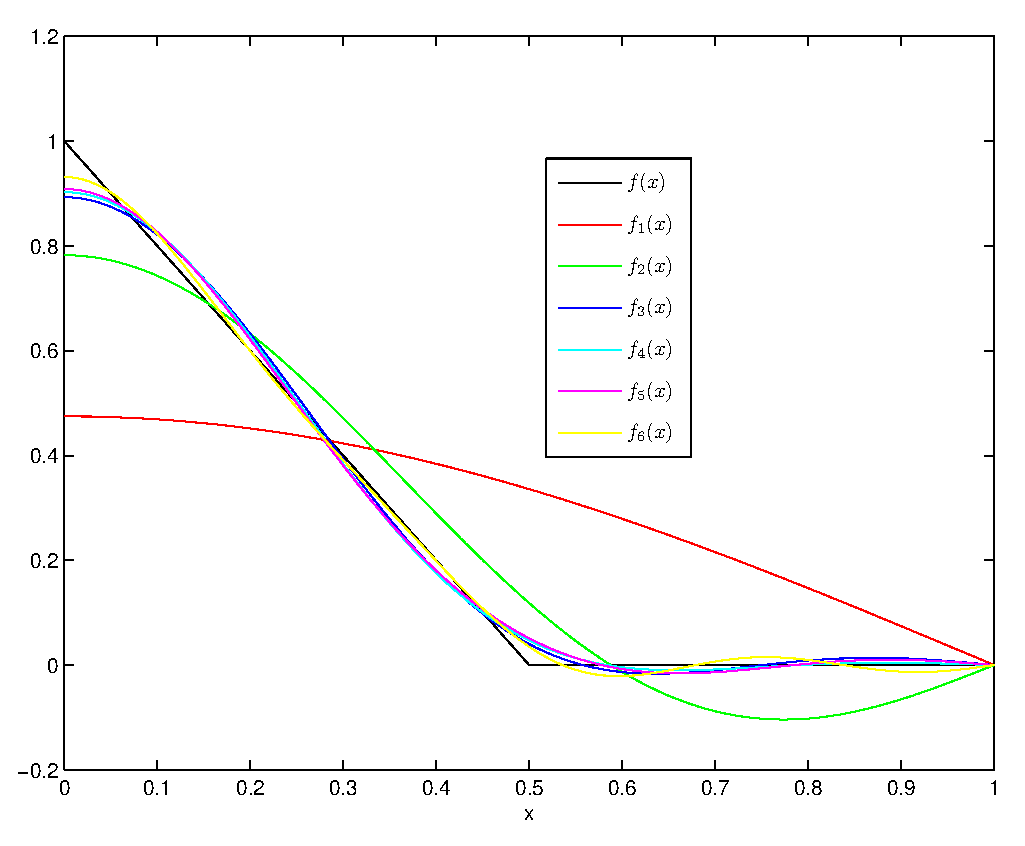
\includegraphics[scale=0.7]{hw72c.eps}\end{center}

The above plot was produced using the following MATLAB code.

\lstinputlisting{HW72c.m}

\item {[4 points]} Now, $\tilde{u}$ is the solution to $L\tilde{u}=f$ and so the spectral method yields the series solution
\[
\tilde{u}(x)=\sum_{n=1}^\infty{\ip{f,\phi_n}\over\lambda_n}\phi_n(x)=\sum_{n=1}^\infty{64\over \left(2n-1\right)^4\pi^4}\left(1-\cos\left({2n-1\over 4}\pi \right)\right)\cos\left({2n-1\over 2}\pi x\right).
\]
\\
\item {[6 points]} Let $\tilde{u}$ be the solution to $L\tilde{u}=f$ and let $w\in C^2[0,1]$ be such that
\[
-w''(x)=0,\quad0<x<1
\]
and
\[
w'(0)=w(1)=1.
\]
Then $u(x)=w(x)+\tilde{u}(x)$ will be such that
\[
-u''(x)=-w''(x)-\tilde{u}''(x)=0+f(x)=f(x);
\]
\[
u'(0)=w'(0)+\tilde{u}'(0)=1+0=1;
\]
and
\[
u(1)=w(1)+\tilde{u}(1)=1+0=1.
\]
Now, the general solution to
\[
-w''(x)=0
\]
is $w(x)=Ax+B$ where $A$ and $B$ are constants. Moreover, $w'(x)=A$ and so $w'(0)=1$ when $A=1$. Hence, $w(x)=x+B$ and so $w(1)=1$ when $B=0$. Consequently,
\[
w(x)=x
\]
and so
\[
u(x)=x+\tilde{u}(x).
\]
We can then use the series solution to $L\tilde{u}=f$ that we obtained in part (c) to obtain the series solution
\[
u(x)=x+\sum_{n=1}^\infty{64\over \left(2n-1\right)^4\pi^4}\left(1-\cos\left({2n-1\over 4}\pi \right)\right)\cos\left({2n-1\over 2}\pi x\right)
\]
to the problem of finding $u\in C^2[0,1]$ such that
\[
-u''(x)=f(x),\quad0<x<1;
\]
\[
u'(0)=u(1)=1.
\]
\\
\item {[4 points]} The best approximation $\tilde{u_N}$ to $\tilde{u}$ from part (d) is
\[
\tilde{u}_N(x)= x+ \sum_{n=1}^N{\ip{f,\phi_n}\over\lambda_n}\phi_n(x)=\sum_{n=1}^N{64\over \left(2n-1\right)^4\pi^4}\left(1-\cos\left({2n-1\over 4}\pi \right)\right)\cos\left({2n-1\over 2}\pi x\right).
\]
The requested plot is below.

\begin{center}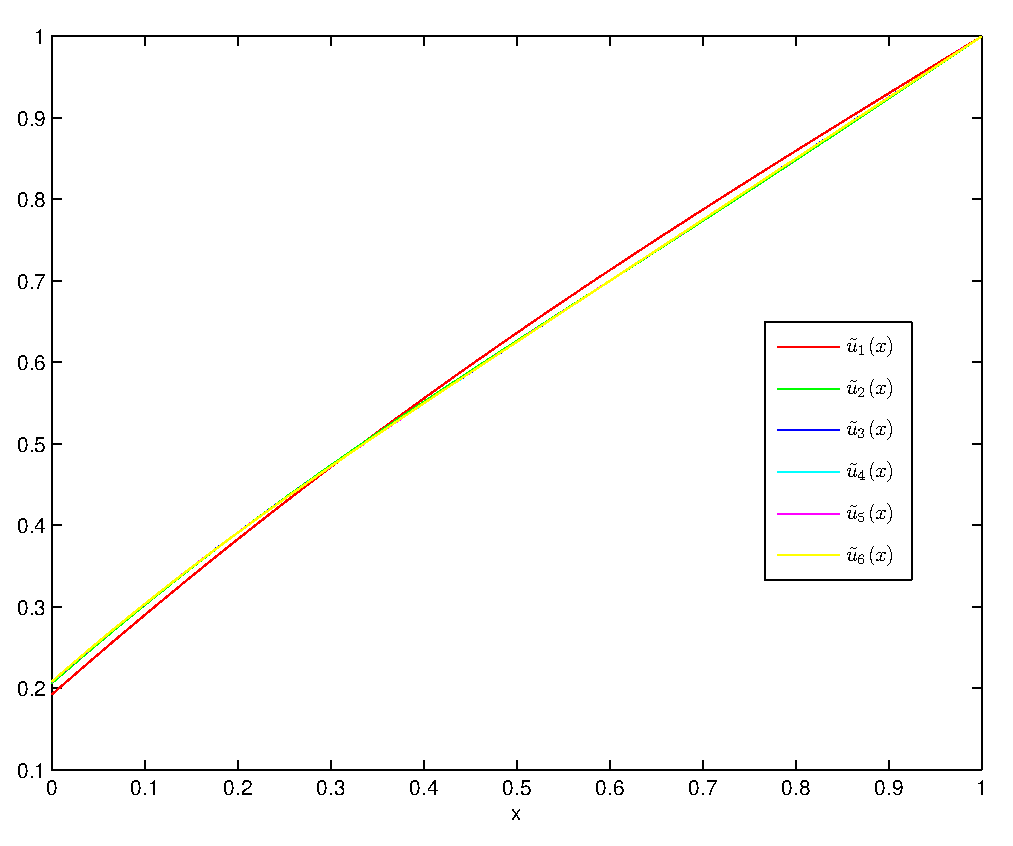
\includegraphics[scale=0.7]{hw72e.eps}\end{center}

The above plot was produced using the following MATLAB code.

\lstinputlisting{HW72e.m}

\end{enumerate}
\end{solution}